% -*-mode: Latex-*-
% !TEX root = thesis.tex
% paper: ...
% authors: simon maurer
%
% file: tbc.tex
% contents: real-time model
% Sccs-Id: %W% %G%
\chapter{Mixed-criticality PNSCs and Time-based Processes}
\label{chap_tcm}
A property of systems in the world of \glspl{cps} is the diversity of components with respect to their criticality and their underlying communication paradigms.
Such systems are called mixed-criticality \glspl{cps}.
They are composed out of components where the consequence of a failure depends on the criticality level of the component.
For example, in a car, a failure of the anti-lock braking system is more critical than the failure of the navigation system.
One challenge of the design and implementation of a mixed-criticality \gls{cps} lies in preventing interference between components of different criticality levels.
This is especially challenging if components with different criticality levels need to interact with each other.
% robotic systems, factory automation, medical devices, process control, real-time speech recognition, embedded computer vision.

Another challenge in the design of \glspl{cps} is the time-criticality of an application.
Traditional software development is based on the best-effort principle where the aspect of time is removed from the control of the programmer.
This lies in contrast to the requirements of a time-critical application where guarantees must be given that a certain piece of code must execute and terminate before a given deadline.
Such deadlines are imposed by the physical world due to physical properties tied to the problem the application aims to solve.

In this chapter I am going to describe how the \gls{pnsc} model (\Chap{\ref{chap_ecm}}) is extended to support mixed-criticality aspects in the event-triggered domain by communication decoupling.
I further introduce timing aspects to the model in order to control communication and triggering rates of processes.
This serves to enable the modelling of safety-critical systems as such systems profit form predictability and stability of communication rates.
The reminder of the chapter is structured as follows:
% To avoid ambiguity, I advocate to use the term \emph{time-critical} systems to describe \emph{hard} real-time systems in particular.
In \Sect{\ref{sect_cci_decoupling}} I discuss the different coupling aspects of communication and describe how communication decoupling in \glspl{pnsc} is achieved in different dimensions.
I use the decoupling mechanisms in conjunction with timers to control communication and execution rates of processes.
This is described in \Sect{\ref{sect_tcm_time}} where two aspects of rate-control are discussed:
First, control on the execution-rate of processes is achieved by removing the event-triggering semantics of a process with the help of communication decoupling and replacing it with a time-triggering semantics where a clock triggers the process execution periodically (\SSect{\ref{sect_tcm_time_tt}}).
Second, the communication rate on individual input ports of processes can be bound to a upper limit to gain control over the used communication bandwidth.
I describe several strategies of how this is achieved in \SSect{\ref{sect_cci_decoupling_rate}}.
In \Sect{\ref{sect_tcm_msg}} I define three different message types and describe their properties, application fields, and how this relates to communication coupling.
In \Sect{\ref{sect_tcm_cci}} I describe \glspl{cci} which summarise the different interaction patterns between processes, based on the triggering semantics of the processes and the types of \glspl*{msg}.
I also provide an example of a mixed-criticality system from the video-processing domain and use the extended \gls{pnsc} model to describe the system.
Finally, in \Sect{\ref{sect_tcm_discussion}} I provide a summary of the chapter, discuss the limitations of the \gls{pnsc} model with respect to time-critical systems, and propose future work related to the topics discussed in this chapter.

%==============================================================================
\section{Communication Decoupling of PNSCs}
\label{sect_cci_decoupling}
One research goal is to provide a platform, suitable for safety-critical services, that is able to perform controlled changes at runtime which is in contrast to the current practice of allowing no changes in safety-critical systems.
Such a platform needs to support the coexistence and segregation of closed subsystems and open subsystems with \emph{\glspl{cci}} between them.
I consider a subsystem as {\em closed} if it doesn't have information flow to or from another subsystem that is essential for the correct functioning of the closed subsystem.
These \glspl{cci} will ensure controlled information flow between closed subsystems and open subsystems such that the closed subsystem cannot be compromised in its correctness in case of misbehaviour by an open subsystem.
\Glspl{cci} avert unwanted coupling of behaviour through the interfaces.

In \Sect{\ref{sect_background_com}} I described communication decoupling in three different dimensions: time, space, and synchronization.
For mixed-criticality systems it is crucial to achieve communication decoupling in order to prevent interference of the lower critical component to the higher critical component.
A \gls{pnsc}, as described in this chapter, relies heavily on synchronous communication.
Synchronous communication is coupled in time because both communication partners need to operate at the same time in order to communicate.
Further, it is also coupled in synchronization because both, the read and the write operation, is blocking.
However, the \gls{pnsc} model achieves decoupling in space due to the presence of channels: processes read from ports (write to ports) without knowing who the producer (the consumer) is.
Communication dependencies are automatically defined through channels that connect to ports with each end.

To make the \gls{pnsc} model suitable for mixed-criticality \glspl{cps} the model needs to be enriched with the possibility to decouple communication in time and synchronisation.% without losing the ability to check for permanent blocking in cases where coupling is not changed.

%------------------------------------------------------------------------------
\subsection{Decoupling PNSCs in Time}
\label{sect_cci_decoupling_time}
To decouple communication in time, a process $N_1$ needs to be able to send a \gls*{msg} to another process $N_2$ without having to wait for $N_2$ to be ready to receive the \gls*{msg} and vice versa.
This can be achieved by introducing a buffer that is independent of the communication partners: a producer can write to the buffer independent of the consumer and the consumer can read from the buffer independent of the producer.
Instead of using a synchronous channel to connect two ports of two processes, a buffering element can be used.
As shown in \Sect{\ref{sect_ecm_example_stream}}, a streaming network with buffered communication can easily be built with the \gls{pnsc} model if each \gls{fifo} buffer (with predefined buffer size) is simply modelled by a process.

Consequently, communication decoupling in time is achieved by introducing an abstraction layer where atomic processes are no longer connected by synchronous channels but by \gls{fifo} channels (each modelled as an atomic \gls{pnsc} process).
An example of such an abstraction is illustrated in \Fig{\ref{fig_cross_procs_dl}} where each double arrow represents an abstraction for a \gls{fifo} buffer.
An example of a \gls{fifo} buffer with two memory spaces is depicted in \Fig{\ref{fig_sia_fifo}}.
I use the notation \channel{double,->}{$a[l]$} to describe a \gls{fifo} buffer $a$ of length $l$.
If the length $l$ is omitted, a default of $l=1$ is assumed.

%------------------------------------------------------------------------------
\subsection{Decoupling PNSCs in Synchronisation}
\label{sect_cci_decoupling_sync}
In an event-triggered communication model, such as the \gls{pnsc} model, the process trigger semantics controls the forward progress of the computation.
Since a read operation on a port is blocking, the process will be triggered by the arrival of a \gls*{msg}, \ie the arrival of a \gls*{msg} initiates the progress in the flow direction of the data.
Due to the blocking write of a \gls{pnsc} process the progression of computation is controlled against the flow direction of the data.
I call this back-pressure.

The blocking communication semantics in a \gls{pnsc} is crucial to ensure event safety in the communication: It is not possible to unintentionally duplicate or lose \glspl*{msg} as processes are blocked as long as the communication partner is not available to exchange information.
% detect permanent blocking situations as described in \Chap{\ref{chap_block}}.
The cost, however, is that blocking creates mutual interference between components.
In case of a mixed-criticality system, it must be possible to punctually remove the blocking semantics of read and/or write operations of a process (decoupling in synchronisation) to prevent interference.

Note that decoupling communication in time does not automatically achieve decoupling in synchronisation.
This is because blocking is possible if no space is available in the buffer for a producer to write to or the buffer is empty and can offer nothing to a consumer.

The blocking semantics of an action $a \in \mathcal{A}_{\descSIA{N}}^I \cup \mathcal{A}_{\descSIA{N}}^O$ in a \gls{sia} $\descSIA{N}$ can be removed by adding a self-loop transition, triggered by action $a$, to each state of the \gls{sia} where action $a$ is not enabled.
This means that the implementation of process $N$ needs to be able to serve the action $a$ in each state of its corresponding \gls{sia} $\descSIA{N}$.
This delegates the problem of decoupling to the implementation of the process which is undesirable because it violates the concept of exogenous coordination.

%------------------------------------------------------------------
\begin{figure}[bht]
    \TopFigSpace
    \centering
    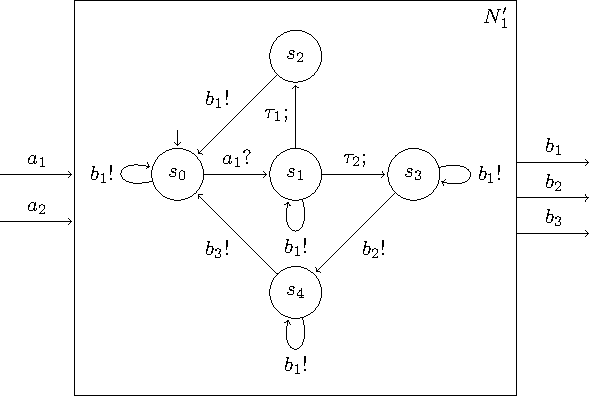
\includegraphics[width=12cm]{fig/sia_decoupled.pdf}
    \CaptionFigSpace
    \caption{An example of a process $N'_1$ where \gls{sia} $\descSIA{N}'_1$ describes the interaction protocol of $N'_1$ with port $b_1$ decoupled in synchronisation.}
    \label{fig_sia_decoupled}
    \BotFigSpace
\end{figure}
%------------------------------------------------------------------
As an example let's consider the process $N_1$ and its corresponding \gls{sia} $\descSIA{N}_1$ as depicted in \Fig{\ref{fig_sia}} where no port is decoupled in synchronisation.
\Fig{\ref{fig_sia_decoupled}} depicts the same situation expect that here, port $b_1$ is decoupled in synchronisation.
% This is indicated by an arrow with an arch symbol at its source.
Due to this decoupling, the \gls{sia} $\descSIA{N}'_1$ has a self-loop transition, triggered by action $b_1 \in \mathcal{A}_{\descSIA{N}'_1}^O$, on each state except state $s_2$ where action $b_1$ is enabled.

This modification of a process and its \gls{sia} is not very convenient because it requires the necessity of different process implementations depending on the context a process is used in.
To avoid this, I introduce a decoupling process $N_D$ with \gls{sia} $\descSIA{N}_D$ as depicted in \Fig{\ref{fig_sia_decoupler}}.
% When composing the \gls{sia} $\descSIA{N}_D$ with the \gls{sia} of a process $N$ (according to the composition operator $\otimes$ as defined in \Def{\ref{def_sia_comp}}), decoupling in synchronisation of a port (in this example port $a$) in process $N$ is achieved.
%------------------------------------------------------------------
\begin{figure}[bht]
    \TopFigSpace
    \centering
    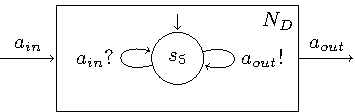
\includegraphics[width=7cm]{fig/sia_decoupler.pdf}
    \CaptionFigSpace
    \caption{An example of a decoupling process $N_D$ and its \gls{sia} $\descSIA{N}_D$ with input $a_{in}$ and output $a_{out}$.}
    \label{fig_sia_decoupler}
    \BotFigSpace
\end{figure}
%------------------------------------------------------------------
The \gls{sia} $\descSIA{N}_D$ of the decoupling process has only one state $s_5$ where it accepts an action $a_{in} \in \mathcal{A}_{\descSIA{N}_D}^I$ and an action $a_{out} \in \mathcal{A}_{\descSIA{N}_D}$.
The decoupling process can never block because each transition in its \gls{sia} is immediately returning to the initial state which allows the process to always consume an input when one is provided and always produce an output when one is required.
In order for a decoupling process to provide an output before it received an input, an initial value must be defined.

%------------------------------------------------------------------
\begin{figure}[bht]
    \TopFigSpace
    \centering
    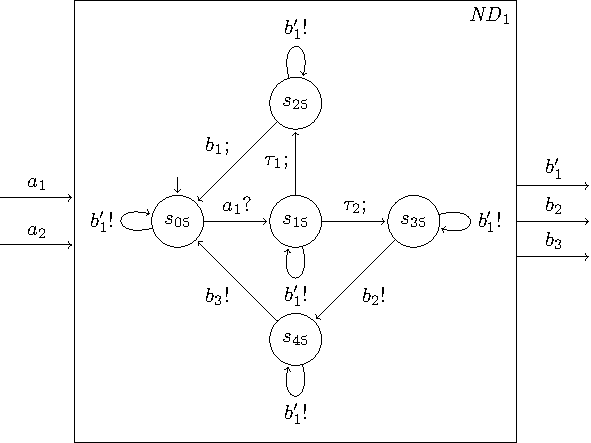
\includegraphics[width=12cm]{fig/sia_decoupled_res.pdf}
    \CaptionFigSpace
    \caption{The resulting abstract process $\mathit{ND}_1$ of the composition $N_1 \otimes N_D$ where \gls{sia} $\descSIA{\mathit{ND}_1} = \descSIA{N}_1 \otimes \descSIA{N_D}$.
    \Gls{sia} $\descSIA{\mathit{ND}_1}$ is syntactically equivalent to \gls{sia} $\descSIA{N}'_1$, depicted in \Fig{\ref{fig_sia_decoupled}}.}
    \label{fig_sia_decoupled_res}
    \BotFigSpace
\end{figure}
%------------------------------------------------------------------
Note that a decoupling process is symmetric.
This means that if a decoupling process $N_D(b_1)$ is used to decouple the output port $b_1$ of process $N_1$, not only does it make the write access of process $N_1$ to port $b_1$ non-blocking but also any read access from the environment to the decoupling process $N_D(b_1)$ becomes non-blocking.
This is illustrated by \Fig{\ref{fig_sia_decoupled_res}} where a decoupling process on channel $b_1$ is composed with process $N_1$ (in order to avoid naming conflicts, the output port of the decoupling process is renamed to $b'_1$).
The resulting process is named $\mathit{ND}_1$ and its corresponding \gls{sia} is defined as $\descSIA{N}_1 \otimes \descSIA{N}_D(b_1)$.
We observe, that the transition $\langle s_{25}, b_1, s_{05} \rangle$ is now triggered by the internal action $b_1$.
Further, we observe that on each state a transition, triggered by the output action $b'_1$, is available which means that the process $\mathit{ND}_1$ is able to serve action $b'_1$ in any state to the environment \ie any write access to the environment and any read access from the environment is decoupled.
Note that \Fig{\ref{fig_sia_decoupled}} and \Fig{\ref{fig_sia_decoupled_res}} are syntactically equivalent.

I conclude that by using a decoupling process on a synchronous channel, the blocking semantics of the channel is removed for the read and the write operation.
Consequently, on a synchronous channel it is only possible to decouple read and write operations simultaneously.
If read and write access must be decoupled individually, the decoupling in synchronisation must be combined with decoupling in time.
I discuss this in detail in \SSect{\ref{sect_cci_decoupling_all}} of this section.
I use the notation \channel{)->}{} to describe a channel where the write access is non-blocking, \channel{->>}{} to describe a channel where the read access is non-blocking, and \channel{)->>}{} to describe a channel where the write and the read access is non-blocking.
As discussed above, a decoupling process, as depicted in \Fig{\ref{fig_sia_decoupler}}, enforces decoupling in synchronisation for read and write access and is, hence, represented as \channel{)->>}{}.
Note that \channel{)->>}{} is only a theoretical construct and in practice decoupling a synchronous channel in synchronisation is equivalent to removing the channel.
This is because the producer and the consumer would need to access the channel at the exact same time and use the physical wire as a buffer to transmit a \gls*{msg}.
In combination with decoupling in time, however, the decoupling process becomes a powerful tool to punctually prevent interference between interacting processes.


%------------------------------------------------------------------------------
\subsection{Decoupling PNSCs in Time and Synchronisation}
\label{sect_cci_decoupling_all}
Achieving decoupling in synchronisation of a process requires either a modification of the process implementation or an additional decoupling process (as depicted in \Fig{\ref{fig_sia_decoupler}}).
However, by combining decoupling in synchronisation with decoupling in time the modification can be applied to the buffer instead of the process.
This allows to connect a process to different types of buffers in order to achieve either input or output decoupling (or both) in synchronization and leave the process implementation unchanged.
In this section, ports are always decoupled in time and space.
When, additionally, a port is decoupled in synchronisation I will simply describe it as \emph{decoupled}.

To achieve this I use the same abstraction as with decoupling in time: synchronous channels are replaced by buffers.
The buffers are not simple \gls{fifo} buffers but have internal logic.
The type of buffer depends on the decoupling semantics of the process ports.
In the following I will describe the different buffer types.

Decoupling an output of a process means that no back-pressure is exert on this output and the process cannot be blocked due to a congestion on the connecting channel.
This is achieved by allowing the process to write to the connecting \gls{fifo} channel, independent of whether there is available space or not.
If the \gls{fifo} buffer is full, the \gls*{msg} in the last buffer space is overwritten by the new \gls*{msg}.
This leads to the potential loss of \glspl*{msg}.
The loss of \glspl*{msg} can be tolerable in certain circumstances.
This will be discussed in more detail in \Sect{\ref{sect_tcm_msg}}.
% This is not problematic if the \gls*{msg} is a state message as defined in \Def{\ref{def_state_msg}} as the presence of the new \gls*{msg} makes the old one obsolete.
% There is no restriction on the number of decoupled outputs of a process, \ie all output ports of a process can be decoupled if necessary.
%------------------------------------------------------------------
\begin{figure}[bht]
    \TopFigSpace
    \centering
    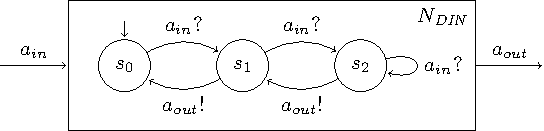
\includegraphics[width=10cm]{fig/sia_cci_in.pdf}
    \CaptionFigSpace
    \caption{An example of a \gls{sia}, modelling a \gls{fifo} buffer of length 2 with a decoupled input $a_{in}$ and an output $a_{out}$.}
    \label{fig_sia_cci_in}
    \BotFigSpace
\end{figure}
%------------------------------------------------------------------
\Fig{\ref{fig_sia_cci_in}} depicts a \gls{fifo} buffer $N_{\mathit{DIN}}$ of length two that is attached to a decoupled output port $a_{in}$ of a process and to a blocking input port $a_{out}$ of another process.
In state $s_0$ the buffer waits for an input action $a_{in}$ to trigger the transition $\langle s_0, a_{in}, s_1 \rangle$.
Once the input is served, in state $s_1$, two transitions are possible.
Either the transition $\langle s_1, a_{out}, s_0 \rangle$ if a consumer is reading from the buffer or the transition $\langle s_1, a_{in}, s_2 \rangle$ if another message is written to the buffer.
In state $s_2$ the buffer is ready to receive any number of \glspl*{msg} due to the transition $\langle s_2, a_{in}, s_2 \rangle$ which models the non-blocking behaviour of the buffer.
I use the notation \channel{double, )->}{$a[l]$} to describe a decoupled \gls{fifo} buffer $a$ of length $l$ where the arch symbol at the source of the arrow indicates the fact that the input of the \gls{fifo} is decoupled in synchronisation and, consequently, \glspl*{msg} can potentially be overwritten and discarded due to the decoupling.

By decoupling an input of a process, this input is excluded from the triggering semantics of the process: a read operation on this port will never block and always return the last \gls*{msg} stored in the connected buffer.
Due to this, decoupling of an input port is only possible for processes with multiple input ports where at least one other input port is triggering the component.
This prevents a component from constantly consuming the same \gls*{msg} without ever being blocked.
Reading from a decoupled input can lead to the duplication of \glspl*{msg}.
The same as the loss of \glspl*{msg}, the duplication of \glspl*{msg} can be tolerated in particular circumstance.
Refer to \Sect{\ref{sect_tcm_msg}} for more information on the subject.
% This is not problematic if the \gls*{msg} is a state message as defined in \Def{\ref{def_state_msg}}.
%------------------------------------------------------------------
\begin{figure}[bht]
    \TopFigSpace
    \centering
    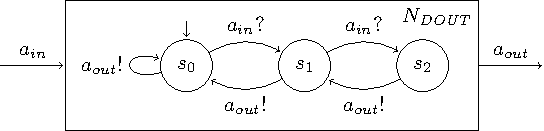
\includegraphics[width=10cm]{fig/sia_cci_out.pdf}
    \CaptionFigSpace
    \caption{An example of a \gls{sia}, modelling a \gls{fifo} buffer of length 2 with input $a_{in}$ and a decoupled output $a_{out}$.}
    \label{fig_sia_cci_out}
    \BotFigSpace
\end{figure}
%------------------------------------------------------------------
An example of a decoupled \gls{fifo} buffer $N_{\mathit{DOUT}}$ of length two is depicted in \Fig{\ref{fig_sia_cci_out}}.
When connected between a producer and a consumer process, such a \gls{fifo} buffer models a decoupled read access of the consumer process to port $a_{out}$ of the \gls{fifo} buffer while the write access of the producer process to the \gls{fifo} buffer (via port $a_{in}$) is blocking.
The initial state $s_0$ allows two transitions:
Either the transition $\langle s_0, a_{in}, s_1 \rangle$ if a \gls*{msg} is written to the buffer or the transition $\langle s_0, a_{out}, s_0 \rangle$ if a consumer is reading from the buffer.
If the latter is the case, the last \gls*{msg} that was written to the buffer is duplicated and the duplicate \gls*{msg} is read by the consumer.
Duplication of the \gls*{msg} ensures that any modification done to the \gls*{msg} by the consumer process does not change the original \gls*{msg} residing in the buffer.

Note that if a \gls*{msg} has never been written to the buffer an empty \gls*{msg} is returned.
I use the notation \channel{double, ->>}{$a[l]$} to describe a decoupled \gls{fifo} buffer $a$ of length $l$ where the double arrow indicates the fact that the output of the \gls{fifo} is decoupled and, consequently, \glspl*{msg} can potentially be duplicated.

%------------------------------------------------------------------
\begin{figure}[bht]
    \TopFigSpace
    \centering
    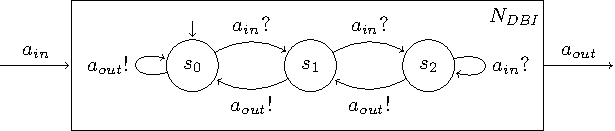
\includegraphics[width=12cm]{fig/sia_cci_bi.pdf}
    \CaptionFigSpace
    \caption{An example of a \gls{sia}, modelling a \gls{fifo} buffer of length 2 with a decoupled input $a_{in}$ and a decoupled output $a_{out}$.}
    \label{fig_sia_cci_bi}
    \BotFigSpace
\end{figure}
%------------------------------------------------------------------
\Fig{\ref{fig_sia_cci_bi}} shows an example of a decoupled \gls{fifo} buffer $N_{\mathit{DBI}}$ of length two that is a combination of the buffers depicted in \Fig{\ref{fig_sia_cci_in}} and \Fig{\ref{fig_sia_cci_out}}.
Such a buffer is used when a decoupled output port of one process is connected to a decoupled input port of another process.
I use the notation \channel{double, )->>}{$a[l]$} to describe a \gls{fifo} buffer $a$ of length $l$ where the input and the output is decoupled.

%==============================================================================
\section{Time-based Component Model of PNSCs}
\label{sect_tcm_time}
In order to give guarantees that a piece of code produces a result before a deadline has passed, one has to know the exact execution time of this piece of code, running on a specific piece of hardware.
However, the execution time of an application, running on a particular hardware platform is not constant because of memory hierarchies, branch predictions, and multi-core designs that are commonly found in modern hardware architectures.
In order to circumvent these problems, huge efforts have been made to compute the \gls{wcet} of an application, running on a specific hardware platform~\cite{wilhelm2008}.

In order to determine the \gls{wcet} of a process, without analysing the behaviour of the environment this process is placed in, a clear separation between communication and computation is necessary~\cite{kopetz2011b}.
This lies in stark contrast to an event-triggered component model, as the one described in \Chap{\ref{chap_ecm}}, where the activation of a process is influenced by the interaction with other processes due to the blocking nature of the communication.
As an alternative, Kopetz proposed the \gls{tta} where a system is decomposed into an assembly of components where each component is triggered according to a fixed schedule.
In \Sect{\ref{sect_background_com}} I gave a short introduction to time-triggered communication which describes one aspect of a \gls{tta}.
In his book~\cite{kopetz2011}, Kopetz discusses time-critical systems and provides an extensive description of \glspl{tta}.

In the following I will discuss two methods to control the execution rate of processes in a \gls{pnsc} by using communication decoupling mechanisms, introduced in \Sect{\ref{sect_cci_decoupling}}, and clock signals.
One method is a \gls{pnsc} version of a time-triggered architecture where the rate of production and consumption of \glspl*{msg} in a \gls{pnsc} is controlled by an element which I call \emph{temporal firewall}.
The other method consists of limiting the production rate of \glspl*{msg} to bound the communication rate to an upper limit.
The former method is described in \SSect{\ref{sect_tcm_time_tt}} and the latter in \SSect{\ref{sect_cci_decoupling_rate}}.

%------------------------------------------------------------------------------
\subsection{Time-triggered Processes in a PNSC}
\label{sect_tcm_time_tt}
In order to change the triggering semantics of a \gls{pnsc}, I introduce the concept of a temporal firewall that allows to enforce a time-triggered semantics on a process or a \gls{pnsc} instead of the sporadic triggering behaviour inherent to \glspl{pnsc}.
A temporal firewall $N_{\mathit{FW}}$ is a \gls{pnsc} process that is connected to a clock signal through port $p_{clk} \in \mathcal{P}_{N_{\mathit{FW}}}$.
The clock signal is oscillating at a constant rate and is causing the temporal firewall to trigger at the rate of the clock signal.
A temporal firewall has another input and a matching output port which are both decoupled in synchronization.
This means that the arrival of a \gls*{msg} at the input port is not triggering the execution of the process, a read access on the input port is non-blocking, and a write access on the output port is non-blocking (see \Sect{\ref{sect_cci_decoupling_sync}}).
% Each decoupled input port of a temporal firewall $N_{\mathit{FW}}$ has a matching decoupled output port, hence $|\mathcal{P}_{N_{\mathit{FW}}}^I \setminus p_{clk} | = |\mathcal{P}_{N_{\mathit{FW}}}^O|$.
Upon the trigger event, caused by the connected clock signal, a temporal firewall consumes a \gls*{msg} from its input port and produces a \gls*{msg} at its output port.
As the input and the output is decoupled, the production and consumption of \glspl*{msg} is independent of the environment of the temporal firewall and it can never be blocked.
%------------------------------------------------------------------
\begin{figure}[bht]\begin{center}
\TopFigSpace
    \centering
    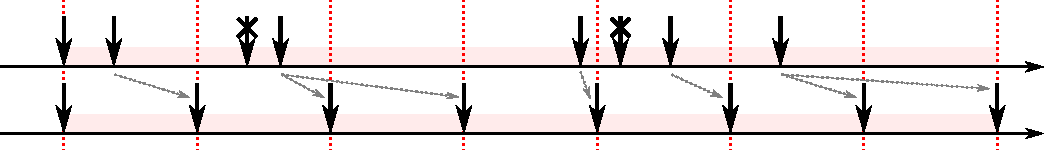
\includegraphics[width=12cm]{fig/rate_control_tt.pdf}
    \CaptionFigSpace
    \caption{An example of the behaviour of a temporal firewall where the upper timeline represents the arrival instances of \glspl*{msg} and the lower timeline represents the release instances of \glspl*{msg}.}
    \label{fig_rate_ctl_tt}
\BotFigSpace
\end{center}\end{figure}
%------------------------------------------------------------------
An example of a behaviour of a temporal firewall is illustrated in \Fig{\ref{fig_rate_ctl_tt}}.
The upper time line represents the arrival instances of \glspl*{msg} at the input of a temporal firewall and the lower timeline represents the release instances of \glspl*{msg} from the output of the temporal firewall.
The vertical dotted lines indicate the rate of the clock that triggers the temporal firewall.
A crossed-out arrow represents a \gls*{msg} that is overwritten by a newer \gls*{msg} (\eg the third \gls*{msg} is overwritten by the fourth and the sixth \gls*{msg} is overwritten by the seventh).

Multiple temporal firewalls can be synchronized by synchronizing the clock signals triggering the temporal firewall.
This is only possible if the clock rate of the synchronized temporal firewalls is equal.
% A set of synchronized temporal firewalls satisfies \Propty{\ref{propty_tf_out}} and \Propty{\ref{propty_tf_in}}:
% \begin{property}[Temporal Firewall Output]
%     \label{propty_tf_out}
%     At the start of a round $r$, each temporal firewall produces exactly one \gls*{msg}.
% \end{property}
% \begin{property}[Temporal Firewall Input]
%     \label{propty_tf_in}
%     Before the start of the next round $r+1$, each temporal firewall consumes exactly one \gls*{msg}.
% \end{property}
% These properties are ensured by the fact that all input and output ports of temporal firewalls are decoupled and that a temporal firewall is periodically triggered by the connected clock signal.

%------------------------------------------------------------------
\begin{figure}[bht]\begin{center}
\TopFigSpace
    \centering
    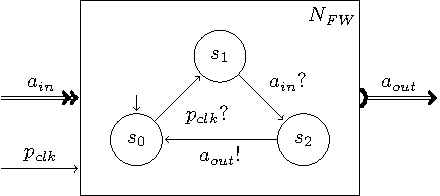
\includegraphics[width=9cm]{fig/sia_firewall_dec.pdf}
    \CaptionFigSpace
    \caption{A temporal firewall with a decoupled port pair $\langle a_{in}, a_{out} \rangle$ and a port $p_{clk}$ which is connected to a clock signal.}
    \label{fig_tcm_tfw}
\BotFigSpace
\end{center}\end{figure}
%------------------------------------------------------------------

A temporal firewall $N_{\mathit{FW}}$ with its corresponding \gls{sia} $\descSIA{N}_{\mathit{FW}}$ is depicted in \Fig{\ref{fig_tcm_tfw}}.
The ports $a_{in}$ and $a_{out}$ are decoupled in synchronisation.
A clock signal is connected to the port $p_{clk}$.
For simplicity I will use the notation \channel{tf,->}{$a(p_{clk})$} to describe a temporal firewall on channel $a$, triggered by the clock signal $p_{clk}$, as depicted in \Fig{\ref{fig_tcm_tfw}}.
Note that decoupled \gls{fifo} channels of length one instead of synchronous channels are connected to the input and output port of a temporal firewall.
% Note that the symbol for a temporal firewall (\channel{tf,->}{$a(p_{clk})$}) and the channel connected to the input and the output of the temporal firewall is represented by a double-lined arrow.
This is because of the following:
While the input and output of a temporal firewall is decoupled in synchronisation by default, the output of the producing process and the input of the consuming process, connected to the temporal firewall, must not necessarily be decoupled in synchronisation.
In order to achieve this separate control of decoupling in synchronisation, decoupling in time is required, hence, buffered channels are used by default.

By connecting all input and output ports of a \gls{pnsc} (or a single process) to synchronized temporal firewalls, a time-triggered behaviour is imposed onto the \gls{pnsc}.
I call such a \gls{pnsc} a time-triggered \gls{pnsc}.
The time-triggered behaviour is enforced because \glspl*{msg} can only reach the time-triggered \gls{pnsc} through temporal firewalls and the temporal firewalls produce \glspl*{msg} at the specified rate which causes the time-triggered \gls{pnsc} to trigger at the specified rate.
Temporal firewalls can be connected to a single process or a \gls{pnsc}.
When connected to a single process, no sporadic triggering is possible because the time-triggered process is completely decoupled from the rest of the network through temporal firewalls.
The \gls{wcet} of the process must be guaranteed to be smaller than the triggering rate imposed by the temporal firewalls.
When connected to a \gls{pnsc}, only processes that communicate with the environment of the time-triggered \gls{pnsc} are decoupled by temporal firewalls.
Other processes inside the time-triggered \gls{pnsc} may still be triggered through sporadic \gls*{msg} transmissions.

%------------------------------------------------------------------
\begin{figure}[bht]\begin{center}
\TopFigSpace
    \centering
    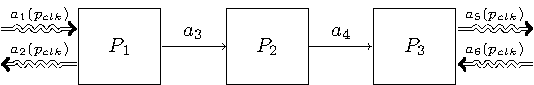
\includegraphics[width=10cm]{fig/procs_tf.pdf}
    \CaptionFigSpace
    \caption{An example of a time-triggered \gls{pnsc} where the \gls{pnsc} is decoupled through temporal firewalls while processes inside the time-triggered \gls{pnsc} trigger sporadically (\eg process $P_2$).}
    \label{fig_tcm_tfnw}
\BotFigSpace
\end{center}\end{figure}
%------------------------------------------------------------------
As an example let's consider the time-triggered \gls{pnsc} depicted in \Fig{\ref{fig_tcm_tfnw}}.
The process $P_1$ interacts through the temporal firewalls $a_1(p_{clk})$ and $a_2(p_{clk})$ with its environment to the left and process $P_3$ interacts through $a_5(p_{clk})$ and $a_6(p_{clk})$ with its environment to the right.
Consequently, the time-triggered \gls{pnsc}, framed by the four temporal firewalls $a_1$, $a_2$, $a_5$, and $a_6$, is decoupled from its environment through the temporal firewalls.
Process $P_2$, however, which is placed inside the time-triggered \gls{pnsc} is not connected to any temporal firewall and is triggering sporadically depending on the arrival of \glspl*{msg} from process $P_1$.
Process $P_3$ is triggered through \glspl*{msg} arriving at the input $a_6$, produced at a rate $p_{clk}$ from a temporal firewall, and through \glspl*{msg} arriving through input port $a_4$, sporadically produced by process $P_2$.
A time-triggered \gls{pnsc} $\mathit{PN}$, framed by synchronized temporal firewalls, must satisfy \Propty{\ref{propty_tt_in}} and \Propty{\ref{propty_tt_out}}.
\begin{property}[Time-triggered Input]
    \label{propty_tt_in}
    At the start of each round $r$, a process $P \in \mathit{PN}$ connected to a temporal firewall via an input port consumes at least one \gls*{msg}.
\end{property}
\begin{property}[Time-triggered Output]
    \label{propty_tt_out}
    Before the start of the next round $r+1$, a process $P \in \mathit{PN}$ connected to a temporal firewall via an output port produces at least one \gls*{msg}.
\end{property}
Note that if more than one \gls*{msg} is consumed or produced by a process $P \in \mathit{PN}$, connected to a temporal firewall, the corresponding port of the process must be decoupled in order to not block the process, given that a temporal firewall produces and consumes exactly one \gls*{msg}.

To tighten the control on the rate of \glspl*{msg} passing in the time-triggered \gls{pnsc} $\mathit{PN}$, each process $P \in \mathit{PN}$ must be framed by synchronized temporal firewalls.
This is illustrated in \Fig{\ref{fig_tcm_ttnw}} which depicts the same example as \Fig{\ref{fig_tcm_tfnw}} but without any sporadic triggering of processes.
%------------------------------------------------------------------
\begin{figure}[bht]\begin{center}
\TopFigSpace
    \centering
    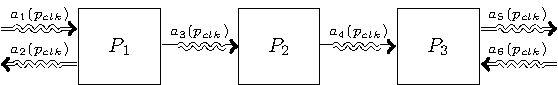
\includegraphics[width=11cm]{fig/procs_tt.pdf}
    \CaptionFigSpace
    \caption{An example of a time-triggered \gls{pnsc} where each process in the \gls{pnsc} is decoupled through temporal firewalls.}
    \label{fig_tcm_ttnw}
\BotFigSpace
\end{center}\end{figure}
%------------------------------------------------------------------
Here, in each clock cycle \glspl*{msg} are passed from one process to the next via temporal firewalls and no sporadic triggering is occurring in the time-triggered \gls{pnsc}.
However, this is only the case if temporal firewalls are synchronized which allows a concatenation of two temporal firewalls, triggered by the same clock rate, to be merged into one (as depicted in \Fig{\ref{fig_tcm_ttnw}}).

If the temporal firewalls, framing the processes are not synchronized, \ie their clock rate differs, temporal firewalls cannot be merged and the time instant of when one temporal firewall produces a \gls*{msg} is not necessarily synchronized with the time instant the neighbouring temporal firewall is consuming a \gls*{msg}.
Consequently, the time instance of passing a message from one process to another is not coordinated.
An example of such a case is depicted in \Fig{\ref{fig_tcm_ttnw_async}} where the processes $P_1$ and $P_2$ are framed by temporal firewalls, each triggered by a different clock rate $clk_1$ and $clk_2$, respectively.
%------------------------------------------------------------------
\begin{figure}[bht]\begin{center}
\TopFigSpace
    \centering
    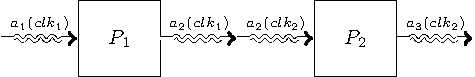
\includegraphics[width=9cm]{fig/procs_tt_async.pdf}
    \CaptionFigSpace
    \caption{An example of a time-triggered \gls{pnsc} where each process in the \gls{pnsc} is decoupled through a temporal firewall with a different clock rate each.}
    \label{fig_tcm_ttnw_async}
\BotFigSpace
\end{center}\end{figure}
%------------------------------------------------------------------

%------------------------------------------------------------------------------
\subsection{Rate-bounded Communication}
\label{sect_cci_decoupling_rate}
To control the bandwidth usage of a communication channel I introduce the concept of rate-bounded communication.
The idea is to introduce a timed guard on a communication channel in order to limit the production rate of \glspl*{msg} in the channel to a specified upper bound.
This bound is specified by the consumer process.
This allows a better prediction of the maximum communication bandwidth demand.
A time interval, called \emph{inter-arrival time}, is used to measure and control the communication rate.
The inter-arrival time describes the elapsed time between the arrival of two consecutive \glspl*{msg}.
If the inter-arrival time of a \gls*{msg} is lower than a specified bound, an action is performed to either delay the \gls*{msg} or to discard it.
Rate-bounded communication is orthogonal to communication coupling and can be applied on all types of coupling configurations of two interacting processes.
However, depending on whether the output of a producer process is decoupled in synchronisation or not, a different method is used to achieve rate-bounded communication.

If the output of the producer process is coupled in synchronisation, \ie the write access to the channel is blocking, back-pressure is used to achieve rate-bounded communication:
The write access not only blocks on write operations if the communication partner is not ready but also if the inter-arrival time of \glspl*{msg} is lower than a specified bound.
% If the output of the producer process is not decoupled, \ie the input-port of the connected \gls{fifo} buffer is not decoupled (\Fig{\ref{fig_sia_fifo}} or \Fig{\ref{fig_sia_cci_out}}), back-pressure is used to achieve rate-bounded communication.
% Hence, the \gls{fifo} buffer not only blocks on write operations if the buffer is full but also if the inter-arrival time of \glspl*{msg} is lower than a specified bound.
Due to the blocking semantics of this rate-control the producing process is not only influenced by the rate of the consuming process but also by the imposed rate-bound on the communication channel.
Let $t_{mia}(p_i)$ describe the minimal inter-arrival time specified on an input port $p_i \in \mathcal{P}^I(N)$ of a process $N$ then the maximum rate $r_{max}(p_i)$ of arriving \glspl*{msg} on port $p_i$ is defined in \Equ{\ref{eq_rate_max}}.
\begin{equation}
    \label{eq_rate_max}
    r_{max}(p_i) = \frac{1}{t_{mia}(p_i)}
\end{equation}
I use the notation \channel{dashed,->}{$p_i(t_{mia})$} to describe a channel $p_i$ bound by the rate $r_{max}(p_i)$ as defined in \Equ{\ref{eq_rate_max}}.

If, on the other hand, the output port of the producer is decoupled in synchronisation, \ie the write access to the channel is non-blocking, discarding of \glspl*{msg} is used to limit the communication rate.
Hence, in addition to discarding \glspl*{msg} if the communication partner is not ready, the corresponding channel also discards \glspl*{msg} if the communication rate is exceeded.
% If, on the other hand, the output port of the producer is decoupled, \ie the input-port of the connected \gls{fifo} buffer is decoupled (\Fig{\ref{fig_sia_cci_in}} or \Fig{\ref{fig_sia_cci_bi}}), discarding of \glspl*{msg} is used to limit the communication rate.
% Hence, in addition to discarding \glspl*{msg} if the buffer is full, the corresponding \gls{fifo} buffer also discards \glspl*{msg} if the communication rate is exceeded.
Due to the discarding of \glspl*{msg} the rate-bound on the communication channel does not impose back-pressure onto the producer process.

In the following I will propose two types of protocols that enforce rate-control without interfering with the producer by discarding \glspl*{msg}:
\begin{enumerate}
    \item The \emph{\gls{mirt}} protocol guarantees that the communication rate at a port $p_i$ never exceeds the maximum rate $r_{max}(p_i)$ as defined in \Equ{\ref{eq_rate_max}}.
        This is ensured by enforcing a minimal time of $t_{mia}$ between the release of two consecutive \glspl*{msg}.
    \item The \emph{\gls{pbrt}} protocol allows to release at maximum one \gls*{msg} per period $t_{max}(p_i)$ at a port $p_i$ but does not enforce a minimal time between two consecutive \glspl*{msg}.
        This allows small peak loads where the time between two consecutive \glspl*{msg} releases is smaller than $t_{mia}$ but ensures that on average the rate of $\frac{1}{t_{mia}(p_i)}$ is not exceeded.
\end{enumerate}

Both types of protocols can either employ a buffer, \ie decouple the communication in time, in order to delay messages and reduce the number of discarded \glspl*{msg} or use a more aggressive strategy and discard \glspl*{msg} straight away if they do not respect the imposed timed guard.
A buffered guard must be an active process because it must be able to release a \gls*{msg} at a later time without blocking the producer process.
Also, a buffered guard increases the latency of a single \gls*{msg} due to the imposed delay.
An unbuffered guard is much simpler because \glspl*{msg} must not be delayed but only discarded if the minimal inter-arrival time is not respected.
This leads to more losses of \glspl*{msg} but the latency of a single \gls*{msg} is not changed.

In the following subsection I will describe each protocol in more detail and give examples.
I use the following notations to identify time values associated to guards:
\begin{description}
    \item[$t_{a}(m)$]
        denotes the arrival time of a \gls*{msg} $m$ at the guard.
    \item[$t_r(m)$]
        denotes the time of the release of a \gls*{msg} $m$ from the guard to its connected \gls{fifo} buffer.\\
        If a \gls*{msg} $m$ is discarded $t_r(m) = \infty$.\\
        For the initial \gls*{msg} $m_0$ I define $t_r(m_0) = t_a(m_0)$.
    \item[$t_{nr}(m)$]
        denotes the minimum time to the next release after the arrival of a \gls*{msg} $m$ at the guard.\\
        For the initial \gls*{msg} $m_0$ I define $t_{nr}(m_0) = t_r(m_0) + t_{mia}$.
    \item[$t_{mia}$]
        denotes the minimum inter-arrival time of two consecutive \glspl*{msg}.
\end{description}

\subsubsection{Rate-control with the MIRT protocol}
The \gls{mirt} protocol accepts \glspl*{msg} only if the minimal inter-arrival time is respected.
Once a \gls*{msg} arrives at the guard, all consecutive \glspl*{msg} arriving within the minimal inter-arrival time interval are discarded.
If the minimal inter-arrival time is respected, \glspl*{msg} are released immediately.
Let $( m_{i-1}, m_i )$ be a sequence of \glspl*{msg} arriving at the guard, then the release time $t_r(m_i)$ of \gls*{msg} $m_i$ is defined in \Equ{\ref{eq_mirt_release}}
\begin{equation}
    t_r(m_i) =
        \begin{cases}
            t_a(m_i) & \quad \text{if } t_a(m_i) \geq t_{nr}(m_{i-1})\\
            \infty   & \quad \text{otherwise}\\
        \end{cases}
    \label{eq_mirt_release}
\end{equation}
and the minimum time of the next release $t_{nr}(m_i)$ after the arrival of \gls*{msg} $m_i$ is defined in \Equ{\ref{eq_mirt_next_release}}
\begin{equation}
    t_{nr}(m_i) =
        \begin{cases}
            t_r(m_i) + t_{mia} & \quad \text{if } t_r(m_i) < \infty\\
            t_r(m_{i-1})       & \quad \text{otherwise}\\
        \end{cases}
    \label{eq_mirt_next_release}
\end{equation}

This is illustrated in the example depicted in \Fig{\ref{fig_rate_ctl_mirt}}.
The arrows on the upper time-line depict the arrival times of the \glspl*{msg}.
Crossed-out arrows represent \glspl*{msg} that are discarded.
The minimal inter-arrival time interval is represented as the lightly coloured area, framed by two dotted lines.
The arrows on the lower time-line represent the release times of \glspl*{msg}.
The timer is activated upon releasing a \gls*{msg} as depicted by the dotted lines in \Fig{\ref{fig_rate_ctl_mirt}}.

\subsubsection{Rate-control with the buffered MIRT protocol}
The buffered \gls{mirt} protocol buffers an arriving \gls*{msg} to delay its progress.
Once the specified minimal inter-arrival time is respected, the delayed \gls*{msg} is released.
\Glspl*{msg} are discarded if multiple \glspl*{msg} arrive within one minimal inter-arrival time interval.
Let $( m_{i-1}, m_i, m_{i+1} )$ be a sequence of \glspl*{msg} arriving at the guard, then the release time $t_r(m_i)$ of \gls*{msg} $m_i$ is defined in \Equ{\ref{eq_bmirt_release}}
\begin{equation}
    t_r(m_i) =
        \begin{cases}
            t_a(m_i)        & \quad \text{if } t_a(m_i) \geq t_{nr}(m_{i-1})\\
            t_{nr}(m_{i-1}) & \quad \text{if } t_a(m_{i+1}) \geq t_{nr}(m_{i-1})\\
            \infty          & \quad \text{otherwise }\\
        \end{cases}
    \label{eq_bmirt_release}
\end{equation}
The minimum time of the next release $t_{nr}(m_i)$ after the arrival of \gls*{msg} $m_i$ is equivalent to the unbuffered \gls{mirt} protocol as defined in \Equ{\ref{eq_mirt_next_release}}.

\Fig{\ref{fig_rate_ctl_bmirt}} represents an example where the same \gls*{msg} arrival times are used as in the previous example but here, a buffered version of the \gls{mirt} protocol is used to release the \glspl*{msg}.
As a consequence, fewer \glspl*{msg} are discarded at the cost of increasing the latency of individual \glspl*{msg}.
If multiple \glspl*{msg} arrive within a minimal inter-arrival time interval, the newest \gls*{msg} is kept and the older ones are discarded (\eg in \Fig{\ref{fig_rate_ctl_bmirt}} the fourth \gls*{msg} replaces the third one and the seventh \gls*{msg} replaces the sixth one).
This lies in contrast to the unbuffered \gls{mirt} protocol where the newer \glspl*{msg} are discarded (see \Fig{\ref{fig_rate_ctl_mirt}}).
This difference is solely due to the presence of the buffer which allows to store the newer message which is not possible in the unbuffered case.
As with the unbuffered \gls{mirt} protocol, also here a timer is activated upon release of a \gls*{msg}.

\subsubsection{Rate-control with the PBRT protocol}
The \gls{pbrt} protocol is based on a periodic timer with period $t_{mia}$.
The policy is to allow the release of at maximum one \gls*{msg} per period.
This ensures that an average rate of $\frac{1}{t_{mia}}$ is not exceeded.
However, it does not specify a maximal rate and allows bursts during a short period, \ie the time between two consecutive \glspl*{msg} can be smaller that the specified period but the average rate can never be exceeded.
Let $( m_{i-1}, m_i )$ be a sequence of \glspl*{msg} arriving at the guard, then the release time $t_r(m_i)$ of \gls*{msg} $m_i$ is equivalent to the unbuffered \gls{mirt} protocol as defined in \Equ{\ref{eq_mirt_release}}.
The minimum time of the next release $t_{nr}(m_i)$ after the arrival of \gls*{msg} $m_i$ is defined in \Equ{\ref{eq_pbrt_next_release}}
\begin{equation}
    t_{nr}(m_i) = (k+1) t_{mia} \text{ with } k \in \mathbb{Z} \ . \ kt_{mia} \leq t_r(m_i) < (k+1)t_{mia}
    \label{eq_pbrt_next_release}
\end{equation}

\Fig{\ref{fig_rate_ctl_pbrt}} depicts an example of a sequence of \glspl*{msg}, released according to the \gls{pbrt} protocol.
Again, the same arrival times of \glspl*{msg} as in the previous examples are used.
In contrast to the \gls{mirt} protocol, the timer is activated periodically, as depicted by the dotted lines.
During a short time the minimal inter-arrival time is violated to compensate for a short burst of \glspl*{msg}.
This allows to reduce the number of discarded \glspl*{msg}.
The violation of the minimal inter-arrival time is highlighted in \Fig{\ref{fig_rate_ctl_pbrt}}.

\subsubsection{Rate-control with the buffered PBRT protocol}
The buffered \gls{pbrt} protocol reduces the number of discarded \glspl*{msg} by using a buffer to delay \glspl*{msg} in order to satisfy the rate requirements.
As with the unbuffered \gls{pbrt} protocol, the timer is periodic with period $t_{mia}$.
An arriving \gls*{msg} can still be discarded if the buffer is already used to delay a \gls*{msg} that arrived before.
In this case the new \gls*{msg} overwrites the old one in the buffer.
Let $( m_{i-1}, m_i, m_{i+1} )$ be a sequence of \glspl*{msg} arriving at the guard, then the release time $t_r(m_i)$ of \gls*{msg} $m_i$ is equivalent to the buffered \gls{mirt} protocol defined in \Equ{\ref{eq_bmirt_release}}.
The minimum time of the next release $t_{nr}(m_i)$ after the arrival of \gls*{msg} $m_i$ is equivalent to the unbuffered \gls{pbrt} protocol as defined in \Equ{\ref{eq_pbrt_next_release}}.

An example of the buffered \gls{pbrt} protocol, applied on a sequence of \glspl*{msg} is depicted in \Fig{\ref{fig_rate_ctl_bpbrt}}.
Also here, the arrival times of the \glspl*{msg} are the same as in the previous examples to allow a comparison between the different approaches.
With this protocol only one \gls*{msg} is discarded.
Again, in contrast to the unbuffered version, the newer \gls*{msg} overwrites the older one and, consequently, the older one is discarded.
This comes at the cost of increasing the latency of individual \glspl*{msg} and allowing a violation of the minimal inter-arrival time.
In \Fig{\ref{fig_rate_ctl_bpbrt}}, the interval where a burst of \glspl*{msg} is accepted is highlighted.

%------------------------------------------------------------------
\begin{figure}[bht]
    \TopFigSpace
    \centering
    \begin{subfigure}[h]{\linewidth}
        \centering
        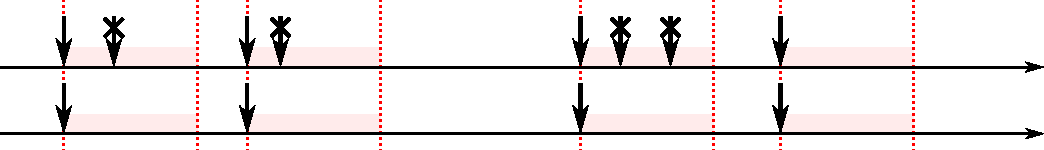
\includegraphics[width=12cm]{fig/rate_control_mirt.pdf}
        \CaptionFigSpace
        \caption{An example of rate-control with the unbuffered \gls{mirt} protocol.}
        \label{fig_rate_ctl_mirt}
        \vspace{1em}
    \end{subfigure}
    \begin{subfigure}[h]{\linewidth}
        \centering
        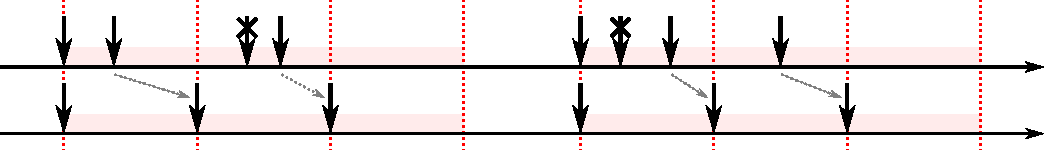
\includegraphics[width=12cm]{fig/rate_control_bmirt.pdf}
        \CaptionFigSpace
        \caption{An example of rate-control with the buffered \gls{mirt} protocol.}
        \label{fig_rate_ctl_bmirt}
        \vspace{1em}
    \end{subfigure}
    \begin{subfigure}[h]{\linewidth}
        \centering
        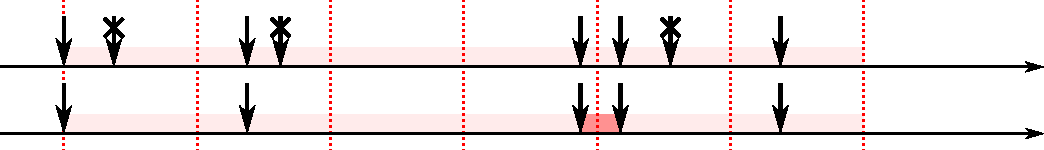
\includegraphics[width=12cm]{fig/rate_control_pbrt.pdf}
        \CaptionFigSpace
        \caption{An example of rate-control with the unbuffered \gls{pbrt} protocol.}
        \label{fig_rate_ctl_pbrt}
        \vspace{1em}
    \end{subfigure}
    \begin{subfigure}[h]{\linewidth}
        \centering
        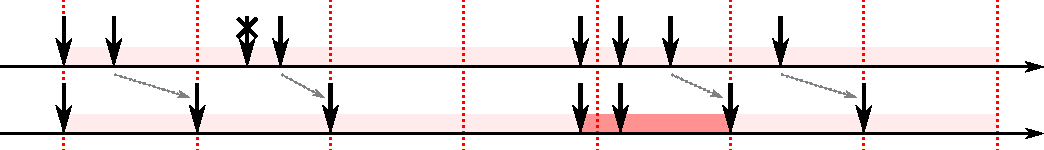
\includegraphics[width=12cm]{fig/rate_control_bpbrt.pdf}
        \CaptionFigSpace
        \caption{An example of rate-control with the buffered \gls{pbrt} protocol.}
        \label{fig_rate_ctl_bpbrt}
    \end{subfigure}
\caption{Examples of rate-control protocols.
In each figure the upper time-line represents the arrival instances of \glspl*{msg} while the lower time-line represents the release instances of \glspl*{msg}.}
    \label{fig_rate_ctl}
    \BotFigSpace
\end{figure}
%------------------------------------------------------------------

%==============================================================================
\section{Message Semantics}
\label{sect_tcm_msg}
In \glspl{pnsc}, communication decoupling in synchronization, as described in \Sect{\ref{sect_cci_decoupling_sync}}, can lead to loss or duplication of \glspl*{msg}.
Depending on the content the \gls*{msg} carries, this can be more or less problematic.
The level of criticality of the transmitted information is an aspect that dictates whether loss or duplication of the information is problematic.
For example, \glspl*{msg} that carry information to perform a monetary transaction have a high criticality and must not be lost.
The loss of a signal of a TV remote control, on the other hand, is inconvenient at most as it can simply be repeated until the transmission is successful.

Apart from the criticality, also the type of the transmitted information plays a crucial role and can alleviate the criticality due to an inherent resilience.
Traditionally, one distinguishes between message types where the content can have information of how to update a subsystem (aka event message) or information about the state of a subsystem (aka state message).
As Kopetz~\cite{kopetz2011d} points out, state messages are well suited for time-triggered systems and event messages for sporadic (event-triggered) systems.
However, as Powell~\cite{powell2002} points out, it is not necessary that a time-triggered system operates solely with state messages nor is it necessary for a sporadic system to operate with event messages.
In the following I will define each message type with respect to message loss and duplication and provide typical application examples for different message types.
I further propose a novel message type, called semi-state message, that has some properties from state messages and some from event messages.
I define a semi-state message in \Def{\ref{def_semi_state_msg}}, a state message in \Def{\ref{def_state_msg}}, and an event message in \Def{\ref{def_event_msg}}.

\begin{definition}[Semi-state Message]
\label{def_semi_state_msg}
A message in a system is called a {\em semi-state message} if it enables a correct system state after a previous message of the same type has been lost and the repeated processing of a single message is tolerated by the system.
\end{definition}

\begin{definition}[State Message]
\label{def_state_msg}
A message in a system is called a {\em state message} if it is a {\em semi-state message} and its arrival makes the processing of non-processed previous messages of the same type obsolete.
\end{definition}

\begin{definition}[Event Message]
\label{def_event_msg}
Every message in a system that is not a semi-state message (and consequently also not a state message) is an {\em event message}.
In case it is not known whether a message is an event or (semi-) state message, it is safe to assume it to be an {\em event message}.
\end{definition}

The loss or duplication of a \gls*{msg} is tolerated by a system if the \gls*{msg} is either of type state message or semi-state message.
In a state message based communication scheme, the producer observes the value of the state variable at a particular time instant and transmits a state message.
An observation is expressed by the triple $<name_{obseravtion}, value, t_{observation}>$.
The transmitted information is useful on its own and no knowledge of a previous transmission is required by the consumer.
A consumer of state messages is only interested in the newest state information of the sender.
Hence, a state message already residing in the communication buffer can be overwritten by a new message without losing any information.
Also, messages can be duplicated without problem as a consumer can perform a non-destructive read to keep the information available for possible further reading operations before a new state message arrives (read access is decoupled in space, time, and synchronisation).
These properties make state messages useful for fault tolerant systems and hence for safety-critical systems.
% Due to this property, message losses and erroneous transmissions may cause bad behaviour only as long as no new correct message is received by the consumer.

In the case of a semi-state message, while the loss or duplication of a \gls*{msg} is tolerated, it is not desirable because the quality of the service might degrade.
Hence, a semi-state message has similar properties as a state message but a system benefits from keeping a history of non-consumed \glspl*{msg}, \ie a \gls*{msg} is not made obsolete with the arrival of a newer \gls*{msg}.

There are cases when (semi-)state messages can not be used or only at high costs.
If, for example, the state variable of the producer is not easily observable or needs to be accessed concurrently (\eg concurrent bank transactions), an infrastructure must be put in place that allows concurrent access.
A message is classified as event message, if the properties of a (semi-)state message, as defined above, are not sufficient to ensure a correct behaviour.
In an event message based communication scheme, an event causes the state variable to change its value.
The producer then transmits the change from the old to the new state variable that was caused by the event.
An event can be expressed by the triple $<name_{event}, \Delta value, t_{event}>$.
% The state variable of the producer can be reconstructed in the consumer by accumulating all event messages.
Generally, it is important that no event message is lost or duplicated and that the order of the messages is preserved.
Event message semantics preserves event safety, \ie prevents losses and duplication of \glspl*{msg}, and is the default assumption of a communication channel, as defined in \Def{\ref{def_channel_msg_semantics}}.
\begin{definition}[Message Semantics of Communication Channel]
\label{def_channel_msg_semantics}
A communication channel that carries only {\em state messages} has a state-message semantics.
A communication channel that carries only {\em state messages} and {\em semi-state messages} has a semi-state-message semantics.
A communication channel that carries {\em event messages} has an event-message semantics.
\end{definition}

It is a design decision of whether the message semantics of a communication channel can be explicitly declared to be of (semi-) state message semantics.
Having a state message or a semi-state message semantics typically depends on the application context.
For example, the stream of video frames of a surveillance camera does have \emph{state semantics} if only life view is required:
Only the most recent picture is relevant but it is important that the most recent picture reflects the current situation of the real world.
But the same video stream would have \emph{semi-state semantics} if it is provided as an online stream that can be consumed over great distances and lossy channels, \ie a good trade-off between a minimum acceptable loss of frames and a minimum acceptable transmission delay is required.
However, if the video is recorded and a later frame-by-frame analysis is required then the video stream would have \emph{event semantics}.

%==============================================================================
\section{Cross-criticality Interfaces}
\label{sect_tcm_cci}
When interconnecting processes with different criticality levels it is important to provide suitable interfaces that allow communication without interference from processes with a lower criticality level towards processes with a higher criticality level.
Further, such interfaces must allow the coexistence of processes with different timing behaviours and message semantics.
I call such interfaces \gls{cci} because they allow interaction between processes of different criticality levels.

Throughout this chapter I introduced communication mechanisms that allow to decouple interactions of processes in space, time, and synchronisation and proposed communication channels that allow to control the communication and execution rate of processes.
In the following list I provide an overview of the different communication channels introduced throughout this chapter and propose new composed channels where multiple properties are combined.
Only combinations are listed that have sensible semantics and a potential use in real applications:
\begin{description}
    \item[\channel{->}{$a$}] depicts a synchronous channel $a$.
        Decoupling of such a channel is not practical (see \Sect{\ref{sect_cci_decoupling_sync}}).
    \item[\channel{double,->}{$a[l]$}] depicts a \gls{fifo} channel $a$ of length $l$.
        Such a channel can be decoupled in synchronisation on its input \channel{double,)->}{$a[l]$}, its output \channel{double,->>}{$a[l]$}, or both \channel{double,)->>}{$a[l]$}.
    \item[\channel{dashed, ->}{$a(t)$}] depicts a synchronous channel $a$ that is bound by a rate defined by $t$.
        Decoupling of such a channel is not practical (see \Sect{\ref{sect_cci_decoupling_sync}}).
    \item[\channel{double,dashed,->}{$a(t)[l]$}] depicts a \gls{fifo} channel $a$ of length $l$ that is bound by a rate defined by $t$.
        Such a channel can be decoupled in synchronisation on its input \channel{double,dashed,)->}{$a(t)[l]$}, its output \channel{double,dashed,->>}{$a(t)[l]$}, or both \channel{double,dashed,)->>}{$a(t)[l]$}.
    \item[\channel{tf,->}{$a(clk)$}] depicts a channel $a$ with an incorporated temporal firewall that is triggered at a rate $clk$.
        Such a channel can be decoupled in synchronisation on its input \channel{tf,)->}{$a(clk)$}, its output \channel{tf,->>}{$a(clk)$}, or both \channel{tf,)->>}{$a(clk)$}.
\end{description}

Table \ref{tab_pattern} lists the same communication channels and provides an overview of properties of each channel.
% The row \emph{channel} lists the different communication channels with their corresponding symbol.
The following properties are described:
\begin{description}
    \item[write] indicates whether the write access to the channel is blocking (block) or non-blocking ($\neg$block), \ie whether the write access is coupled or decoupled in synchronisation.
    \item[read] indicates whether the read access to the channel is blocking (block) or non-blocking ($\neg$block), \ie whether the read access is coupled or decoupled in synchronisation.
    \item[lossy] indicates whether \glspl*{msg} can potentially be lost (yes) or not (no).
    \item[copy] indicates whether \glspl*{msg} can potentially be duplicated (yes) or not (no).
    \item[rate] describes the communication rate of transmitted \glspl*{msg}.
    \item[buffer] indicates whether the channel is buffered (yes) or unbuffered (no), \ie whether the channel is decoupled or coupled in time.
    \item[event] indicates if the channel supports event messages (yes) or if (semi-)state messages are better suited (no).
\end{description}

The table shows that imposing a fixed communication rate with a temporal firewall, as described in \Sect{\ref{sect_tcm_time_tt}}, is only suitable for (semi-)state messages because loss or duplication of \glspl*{msg} can happen independently of communication coupling.
The decision of whether a read or write access on a temporal firewall should be blocking or non-blocking depends solely on the intended progression control of the process:
It might be desirable to block a producer process, connected to a temporal firewall, until the produced \gls*{msg} is consumed by the temporal firewall in order to avoid unnecessary computation efforts of the producer process.
On the other hand it might be desirable to allow the producer process to refine its result and overwrite the previous output.
The latter requires decoupling in synchronisation to make the write access to the channel non-blocking.

%------------------------------------------------------------------
\begin{table}[bht]
    \renewcommand{\arraystretch}{1.3}
    \TopTabSpace
    \caption{A list of the properties of communication channels, formed from different combinations of communication patterns.}
    \label{tab_pattern}
    \CaptionTabSpace
    \centering
    % \normalsize
    % \small
    \begin{tabular}{c|*{7}{|c}}
                                  & write       & read        & lossy & copy & rate     & buffer & event \\
        \hline
        \hline
        \channel{->}{}            & block       & block       & no    & no   & sporadic & no     & yes   \\
        \hline
        \channel{fifo, ->}{}      & block       & block       & no    & no   & sporadic & yes    & yes   \\
        \channel{fifo, ->>}{}     & block       & $\neg$block & no    & yes  & sporadic & yes    & no    \\
        \channel{fifo, )->}{}     & $\neg$block & block       & yes   & no   & sporadic & yes    & no    \\
        \channel{fifo, )->>}{}    & $\neg$block & $\neg$block & yes   & yes  & sporadic & yes    & no    \\
        \hline
        \channel{tb, ->}{}        & block       & block       & no    & no   & bounded  & no     & yes   \\
        \hline
        \channel{tb,fifo, ->}{}   & block       & block       & no    & no   & bounded  & yes    & yes   \\
        \channel{tb,fifo, ->>}{}  & block       & $\neg$block & no    & yes  & bounded  & yes    & no    \\
        \channel{tb,fifo, )->}{}  & $\neg$block & block       & yes   & no   & bounded  & yes    & no    \\
        \channel{tb,fifo, )->>}{} & $\neg$block & $\neg$block & yes   & yes  & bounded  & yes    & no    \\
        \hline
        \channel{tf,->}{}         & block       & block       & yes   & yes  & fixed    & yes    & no    \\
        \channel{tf,->>}{}        & block       & $\neg$block & yes   & yes  & fixed    & yes    & no    \\
        \channel{tf,)->}{}        & $\neg$block & block       & yes   & yes  & fixed    & yes    & no    \\
        \channel{tf,)->>}{}       & $\neg$block & $\neg$block & yes   & yes  & fixed    & yes    & no    \\
    \end{tabular}
    \BotTabSpace
\end{table}
%------------------------------------------------------------------

The attributes of \emph{sporadic} communication channels are equivalent to the attributes of channels with a \emph{bounded} communication rate when considering the same coupling configuration (with the exception of the \emph{rate} attribute).
This means that bounding the communication rate, as described in \Sect{\ref{sect_cci_decoupling_rate}}, only influences the communication rate but does not change the communication coupling behaviour of a channel.

%------------------------------------------------------------------------------
\subsection{Mixed-criticality Network with CCIs}
\label{sect_tcm_cci_example}
In this section I describe a mixed-criticality video processing application that relies on different communication channels, introduced in this chapter.
The basic principle of the application is to record video images with a camera, perform two independent video processing tasks on the video frames, and display the result on a screen.
One of the two video processing tasks is of high criticality and must be guaranteed to perform correctly while the other step is of low criticality as it only improves the result but is not absolutely necessary.
The challenge of this application is that the lower critical processing task is more complicated and requires more resources than the high criticality task and it must be ensured that the low criticality task does not interfere with the high criticality task.

The example depicted in Figure \ref{fig_mc_pnsc_ex} shows a \gls{pnsc} that models such an image processing application.
The process $P_{cam}$ produces \glspl*{msg} containing video frames and communicates them to the process $P_{copy}$.
The process $P_{copy}$ copies the arriving \glspl*{msg} to each of two connected channels at its output ports.
The upper channel connects to the process $P_{filter}$ where the video frames, consumed via its input port, are processed and then sent to the output port.
The lower channel connects to the process $P_{fd}$ where a complex feature detection algorithm is executed on the video frames.
The process $P_{merge}$ consumes \glspl*{msg} from the processes $P_{filter}$ and $P_{fd}$ and merges the two video frames into one.
\Glspl*{msg} with the merged video frames are then transmitted to the process $P_{screen}$ where the video is displayed.
%------------------------------------------------------------------
\begin{figure}[bht]\begin{center}
\TopFigSpace
    \centering
    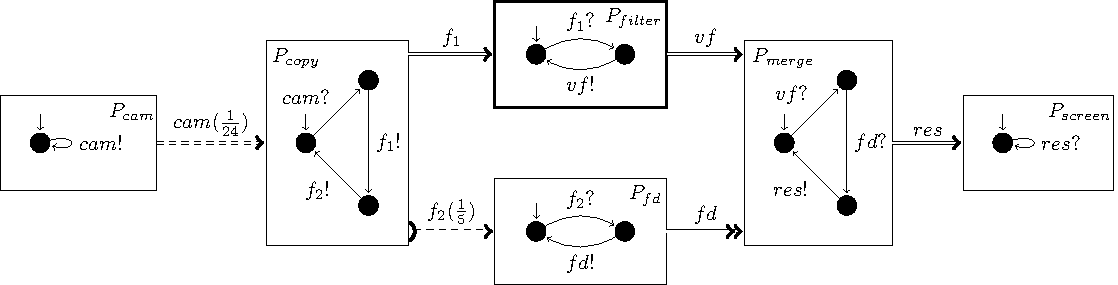
\includegraphics[width=\linewidth]{fig/mc_pnsc_ex.pdf}
    \CaptionFigSpace
    \caption{An example of a mixed-criticality video processing application where ports are decoupled in synchronisation to prevent interference from the low critical process $P_{fd}$ towards the high criticality process $P_{filter}$.}
    \label{fig_mc_pnsc_ex}
\BotFigSpace
\end{center}\end{figure}
%------------------------------------------------------------------

All communication channels are buffered to allow a variation in the production rate of the processes.
The channel $cam$, connecting process $P_{cam}$ with process $P_{copy}$, is bounded to a maximum rate of $\frac{1}{24}$ which is sufficient for this particular video processing application.
% Back-pressure limits the production rate of the producing processes while \gls{fifo} buffers allow a variation of the production rate.
The process $P_{filter}$ is of high criticality (the box with the thick border in \Fig{\ref{fig_mc_pnsc_ex}}) and process $P_{fd}$ is of low criticality, hence, it must be ensured that $P_{fd}$ is not interfering with $P_{filter}$.
To achieve this, first, the output $f_2$ of process $P_{copy}$ is decoupled in synchronisation to prevent back-pressure from the low-criticality process $P_{fd}$.
Consequently, process $P_{copy}$ cannot be blocked by process $P_{fd}$ which prevents indirect interference from process $P_{fd}$ towards process $P_{filter}$.
Second, the input $fd$ of process $P_{merge}$ is decoupled in synchronisation to prevent a blocking read access from process $P_{merge}$ to this channel which prevents any indirect interference from process $P_{fd}$ towards process $P_{filter}$ via process $P_{merge}$.

Additionally, the channel $f_2$ is bounded to a maximum rate of $\frac{1}{5}$ to prevent the execution of process $P_{fd}$ at a faster rate than is useful for this particular application.

%==============================================================================
\section{Discussion}
\label{sect_tcm_discussion}
A main contribution of this chapter is the modular approach to punctually remove communication coupling to prevent interference.
It is especially useful that this is achieved without changing the specification of a process but solely by changing the communication channels the process interacts with.
This modularity allows to reuse a process in different contexts without any need for the process to be aware of the context it is placed in.

For future work, it might be interesting to investigate if in a network of processes, channel types can be chosen automatically to prevent interference where necessary, depending on the criticality level of individual processes.

With respect to time-triggered \glspl{pnsc}, as temporal firewalls can be connected independently to processes, it is possible to enforce a time-triggered semantics on individual processes in a \gls{pnsc} or on a \gls{pnsc} as a whole.
In the former case each \gls*{msg} in the \gls{pnsc} is transmitted according to the time-triggered communication semantics.
In the latter case, processes inside the time-triggered \gls{pnsc} communicate sporadically whereas a process interacting with the environment of the \gls{pnsc} follows a time-triggered communication scheme.
Such time-triggered \glspl{pnsc} can be useful when designing an application for a many-core architecture, \eg 256 cores, where several clusters of cores, \eg 16 clusters, communicate via shared memory (use a sporadic communication scheme) while the clusters are interlinked by a \gls{noc} (use the time-triggered communication scheme)\footnote{The Kalray MPPA\textsuperscript{\textregistered}-256 (Andey) is an example of such a processor.}.
De Dinechin \etal propose a \gls{rts} for such an architecture that supports \ia a time-triggered and a \gls{kpn} execution model~\cite{deDinechin2013}.

In \Sect{\ref{sect_tcm_time_tt}} I mentioned that a time-triggered \gls{pnsc} must satisfy \Propty{\ref{propty_tt_in}} and \Propty{\ref{propty_tt_out}} in order to be valid.
It is rather complex to provide sufficient requirements to guarantee these properties and an extensive investigation of this topic is required.
The bulk of this work is postponed to future work.
I will, however, give an overview of the work that needs to be done to achieve this goal:
Both properties rely on the requirement that within one round each process of the time-triggered \gls{pnsc} has completed its execution.
This can only be guaranteed if the \gls{wcet} of the \gls{pnsc} is known and is guaranteed to be smaller than the specified time to complete one round.
The \gls{wcet} of the \gls{pnsc} depends on the network topology of the \gls{pnsc} and the \gls{wcet} of each process in the \gls{pnsc}.
Further, the \gls{wcet} of a process depends on the decisions made within the process and how it interacts with its environment.
The \gls{sia} of a \gls{pnsc} process describes the interaction protocol with its environment.
By extending a \gls{sia} with \gls{wcet} annotations on each action and using the network description provided by the \gls{pnsc} model, it should be possible to check whether a time-triggered \gls{pnsc} satisfies \Propty{\ref{propty_tt_in}} and \Propty{\ref{propty_tt_out}}.

% Regulations and requirements are increasingly strict with increasing criticality of the application, \ie the bigger the consequences of missing deadlines, the higher the criticality of the system.
% Hence, with increasing system criticality, more effort has to be spent to guarantee timings.
% This leads to the situation where. \eg in the aeroplane industry, costs for testing whether a software is guaranteed to perform correctly on a hardware platform are so high that it is not practical to ever change the hardware type during the lifespan of a product.
% Consequently, aeroplane constructors stockpile huge amounts of hardware platforms in order to have replacement parts to perform maintenance during the lifespan of a product.
% In his paper on design challenges of \gls{cps}~\cite{lee2008}, Lee discusses this problem and lists several approaches that might help to contribute to a solution.

% coordination languages as a solution for this problem
% an approach that allows to loosen the tight coupling between a software application and its hardware platform when it comes to time-criticality.


%==============================================================================
\section{Chapter Summary}
\label{sect_tcm_summary}
In this chapter I extended the \gls{pnsc} model with communication channels that allow to change the communication coupling and triggering semantics of connected processes.
This enables the \gls{pnsc} model to describe mixed-criticality systems where processes with different criticality levels can interact without interference.
While the example in \Fig{\ref{fig_mc_pnsc_ex}} describes a system with two criticality levels, the model is not limited to two criticality levels.
The decoupling element is used to prevent interference between any two criticality levels and, thus, can be applied on multiple levels.

I further extended the \gls{pnsc} model with two rate-controlled channels that allow to model time-critical systems:
First, a fixed-rate communication channel, called a temporal firewall, can be used to enforce time-triggered semantics of a process.
Second, a rate-bound communication channel serves to limit the communication rate to an upper bound.
This increases the predictability of the required bandwidth and allows to distribute the available bandwidth where it is needed.

Finally, I proposed \glspl{cci} where combinations of these concepts are put together and I discussed the properties of the \glspl{cci}, in particular with respect to different message semantics.
In this context I introduced a novel message type, namely \emph{semi-state} messages which which has some properties of state messages and some properties of event messages.
